\chapter{Experiment 0}
\section{Introduction}
This project investigates the application of reinforcement learning algorithm and neural networks to the problem of producing an agent that can play board games. With the help of neural network and concepts of artificial intelligence we want to build the framework in which the agent by itself would be able to create the optimal policy in a faster way. So experiments involve developing agent for 2048 game. Moreover 2048 is one player game and simpler to test algorithms.

\section{2048 experiment}
In this experiment $\epsilon$-greedy algorithm has been explored and the algorithm for that is as follows:

\begin{steps}
 \item Choose $\epsilon$ from [0,1] 
 \item $x$ $\sim$ $uniform(0,1)$
 \item if $x$ $<$ $\epsilon$:
 	Choose random action\\
 	else:
 	Exploit it by taking most rewarding action from current state
\end{steps}

\section{Model Architecture}

\begin{figure}
 	[!htb]\centering
    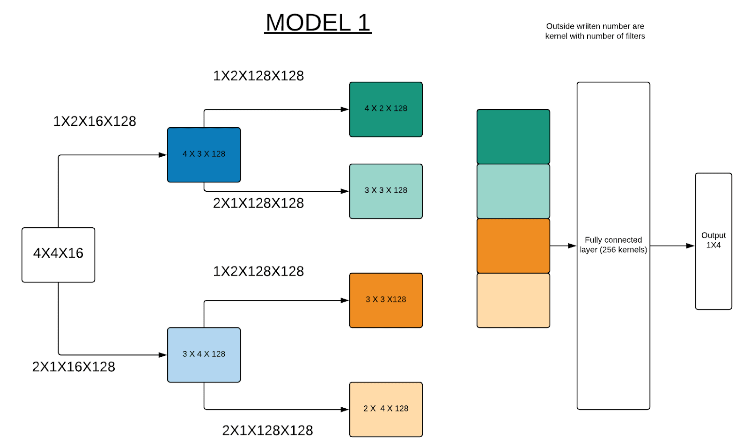
\includegraphics[width=4in]{images/model1.png}
    \caption{Simple neural network with 4*4*16 as board state}
  \label{fig:phase}
  \end{figure}

\begin{figure}
 	[!htb]\centering
    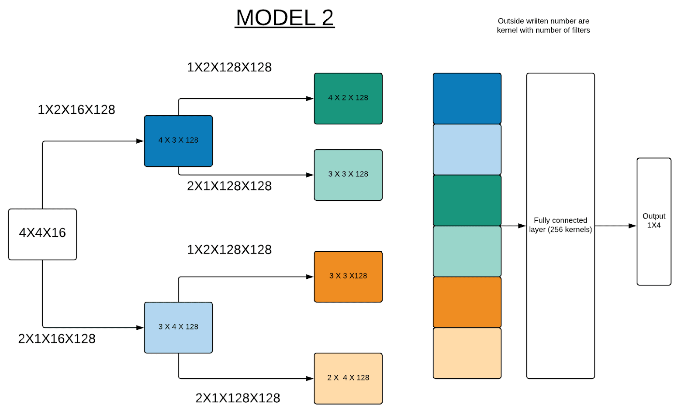
\includegraphics[width=4in]{images/model2.png}
    \caption{More complex neural network than model 1 because last layer is directly connected to two previous layers}
  \label{fig:phase}
  \end{figure}
 
\section{Results and conclusion}
After analyzing loss function and board reaching to maximum number is compared and averaged over 20 number of games, both got similar results and loss function for both network was same. So the architecture of neural network does not affect much.
